\begin{figure}[ht]
  \centering
  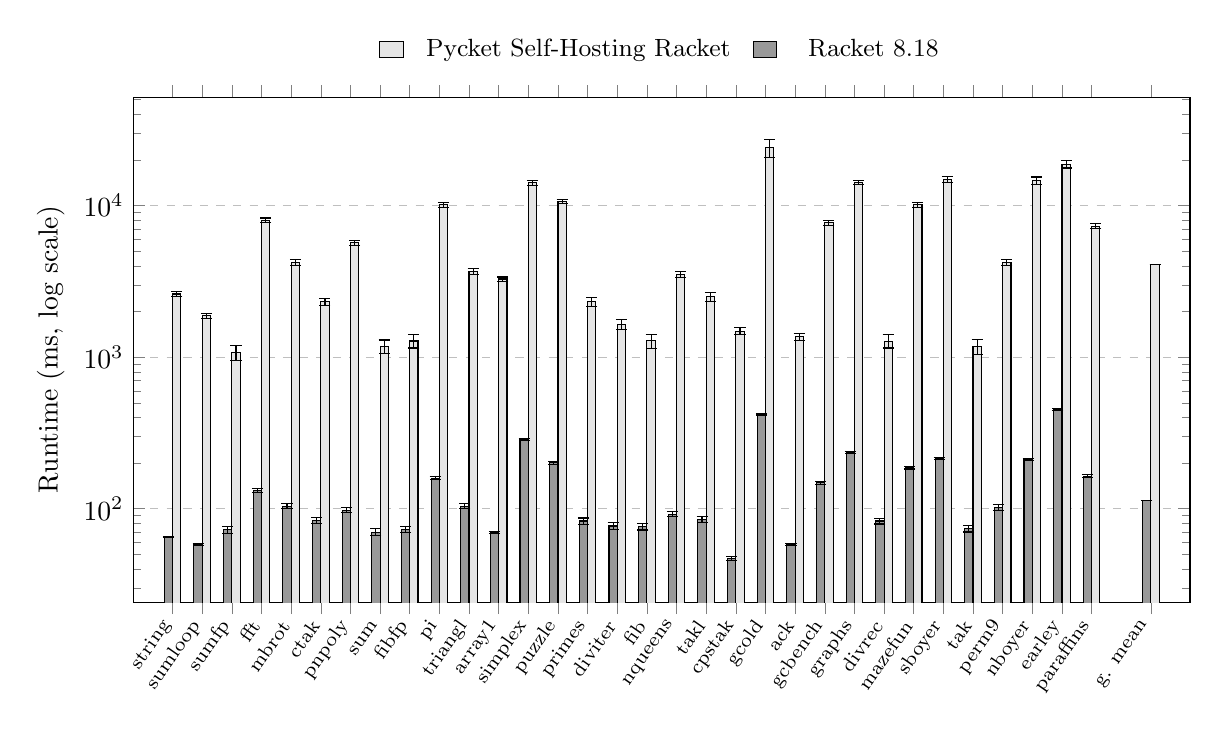
\begin{tikzpicture}
  \begin{axis}[
    ybar,
    bar shift=0pt,
    bar width=3pt,
    width=15cm,
    height=8cm,
    ymode=log,
    log basis y=10,
    scaled y ticks=false,
    ylabel={Runtime (ms, log scale)},
    symbolic x coords={
      string,sumloop,sumfp,fft,mbrot,ctak,pnpoly,sum,fibfp,pi,triangl,array1,
      simplex,puzzle,primes,diviter,fib,nqueens,takl,cpstak,gcold,ack,gcbench,
      graphs,divrec,mazefun,sboyer,tak,perm9,nboyer,earley,paraffins,,g. mean},
    xtick=data,
    xticklabel style={rotate=55,anchor=east,font=\scriptsize},
    enlarge x limits=0.04,
    ymajorgrids=true,
    grid style=dashed,
    legend style={
        at={(0.5,1.05)},
        anchor=south,
        legend columns=2,
        column sep=6pt,
        draw=none,
        fill=none,
        font=\small,
        /tikz/column 2/.style={anchor=west},
    },
    legend image code/.code={
        \draw[#1,fill=#1] (-0.15cm,-0.10cm) rectangle (0.15cm,0.10cm);
    },
  ]

  %────────────────────────  Pycket Self‑hosting  ────────────────────────
  \addplot[
    ybar,
    fill=gray!20,
    draw=black,
    bar shift=+1.5pt,
    error bars/.cd,
      y dir=both,
      y explicit,
  ] coordinates {
    (string,2609)     +- (0,97.68)
    (sumloop,1878)    +- (0,68.15)
    (sumfp,1078)      +- (0,122.32)
    (fft,8008)        +- (0,275.71)
    (mbrot,4228)      +- (0,179.65)
    (ctak,2316)       +- (0,134.85)
    (pnpoly,5668)     +- (0,187.85)
    (sum,1176)        +- (0,121.88)
    (fibfp,1279)      +- (0,129.59)
    (pi,10137)        +- (0,386.88)
    (triangl,3694)    +- (0,165.33)
    (array1,3278)     +- (0,102.17)
    (simplex,14105)   +- (0,458.38)
    (puzzle,10684)    +- (0,350.35)
    (primes,2327)     +- (0,157.48)
    (diviter,1643)    +- (0,124.55)
    (fib,1280)        +- (0,137.37)
    (nqueens,3516)    +- (0,171.67)
    (takl,2508)       +- (0,167.17)
    (cpstak,1485)     +- (0,74.69)
    (gcold,24044)     +- (0,3362.14)
    (ack,1367)        +- (0,71.07)
    (gcbench,7699)    +- (0,306.06)
    (graphs,14249)    +- (0,409.29)
    (divrec,1276)     +- (0,126.86)
    (mazefun,10152)   +- (0,382.54)
    (sboyer,14821)    +- (0,644.38)
    (tak,1177)        +- (0,131.35)
    (perm9,4229)      +- (0,195.00)
    (nboyer,14576)    +- (0,865.64)
    (earley,18704)    +- (0,996.70)
    (paraffins,7313)  +- (0,266.17)
    % empty spacer: no coordinate
    (g. mean,4060)    +- (0,0)
  };

  %────────────────────────────  Racket 8.18  ────────────────────────────
  \addplot[
    ybar,
    fill=gray!80,
    draw=black,
    bar shift=-1.5pt,
    error bars/.cd,
      y dir=both,
      y explicit,
  ] coordinates {
    (string,65)     +- (0,0.77)
    (sumloop,58)    +- (0,0.79)
    (sumfp,73)      +- (0,3.88)
    (fft,132)       +- (0,3.75)
    (mbrot,104)     +- (0,3.63)
    (ctak,84)       +- (0,3.86)
    (pnpoly,98)     +- (0,3.73)
    (sum,70)        +- (0,3.60)
    (fibfp,73)      +- (0,3.75)
    (pi,159)        +- (0,4.06)
    (triangl,104)   +- (0,3.70)
    (array1,70)     +- (0,0.88)
    (simplex,288)   +- (0,4.18)
    (puzzle,201)    +- (0,4.53)
    (primes,83)     +- (0,3.84)
    (diviter,77)    +- (0,4.08)
    (fib,76)        +- (0,3.64)
    (nqueens,92)    +- (0,3.57)
    (takl,85)       +- (0,3.41)
    (cpstak,47)     +- (0,1.34)
    (gcold,420)     +- (0,4.32)
    (ack,58)        +- (0,0.79)
    (gcbench,148)   +- (0,3.91)
    (graphs,234)    +- (0,3.70)
    (divrec,83)     +- (0,3.63)
    (mazefun,187)   +- (0,3.94)
    (sboyer,214)    +- (0,3.90)
    (tak,74)        +- (0,3.70)
    (perm9,102)     +- (0,4.09)
    (nboyer,211)    +- (0,3.75)
    (earley,451)    +- (0,5.25)
    (paraffins,164) +- (0,3.95)
    % empty spacer: no coordinate
    (g. mean,114)   +- (0,0)
  };

  \legend{Pycket Self‑Hosting Racket, Racket 8.18}
  \end{axis}
  \end{tikzpicture}
  \caption{Program‑expansion performance. Pycket with Self‑hosting with and without extended green variables optimization vs.\ Racket 8.18 — lower is better.}
  \label{fig:crossbenchmark-expansion-times-vs-R-green-vars}
\end{figure}
